% This is HBBNC and HBC
\label{section:HBBNC}
\label{section:HBC}
\section{Abstract}
\section{Introduction}
\begin{itemize}
	\item How is gas adsorption on molecules interesting?
		\subitem oxygen transport in blood, more examples?
	\item Has gas adsorption played a role on PAH?
\end{itemize}

\section{The molecule}
Coronene ($C_{24}H_{12}$, known as [6]circulene or super benzene) is a polycyclic aromatic hydrocarbon made of six carbon rings to form a molecule reminiscent of a small graphene flake. It belongs to the family of circulenes where a central polygon is enclosed by different numbers of fused benzenoids. For example [5]circulene (corannulene), [6]circulene (coronene), [7]circulene,[2][3][4][5] and higher orders could be synthesized and show different conformation. While species with 5 or 7 benzene rings are bowl shaped, coronene is flat.

\begin{figure}[h!]\centering
	\subfigure[HBC]{
		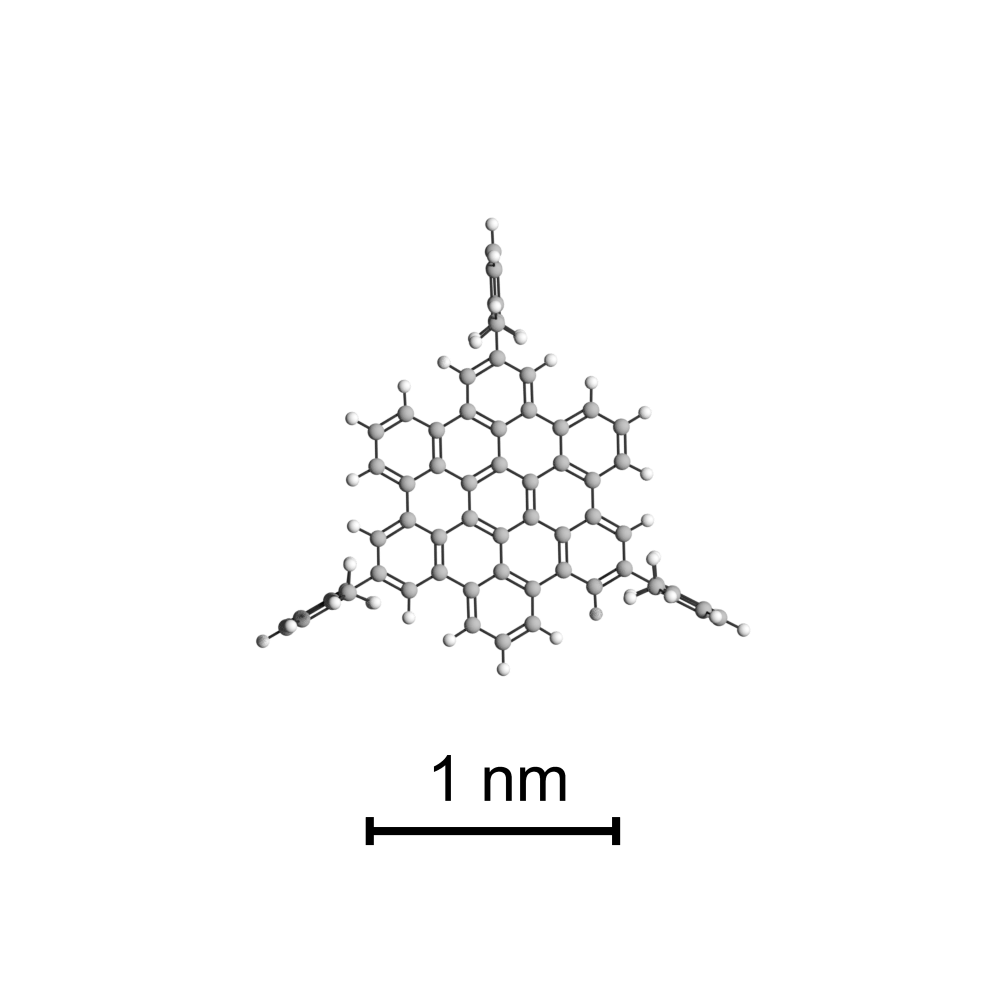
\includegraphics[width=0.45\textwidth]{./images/molecules/HBC-scalebar}
		\label{fig:HBC}
	} \quad
	\subfigure[HBBNC]{
		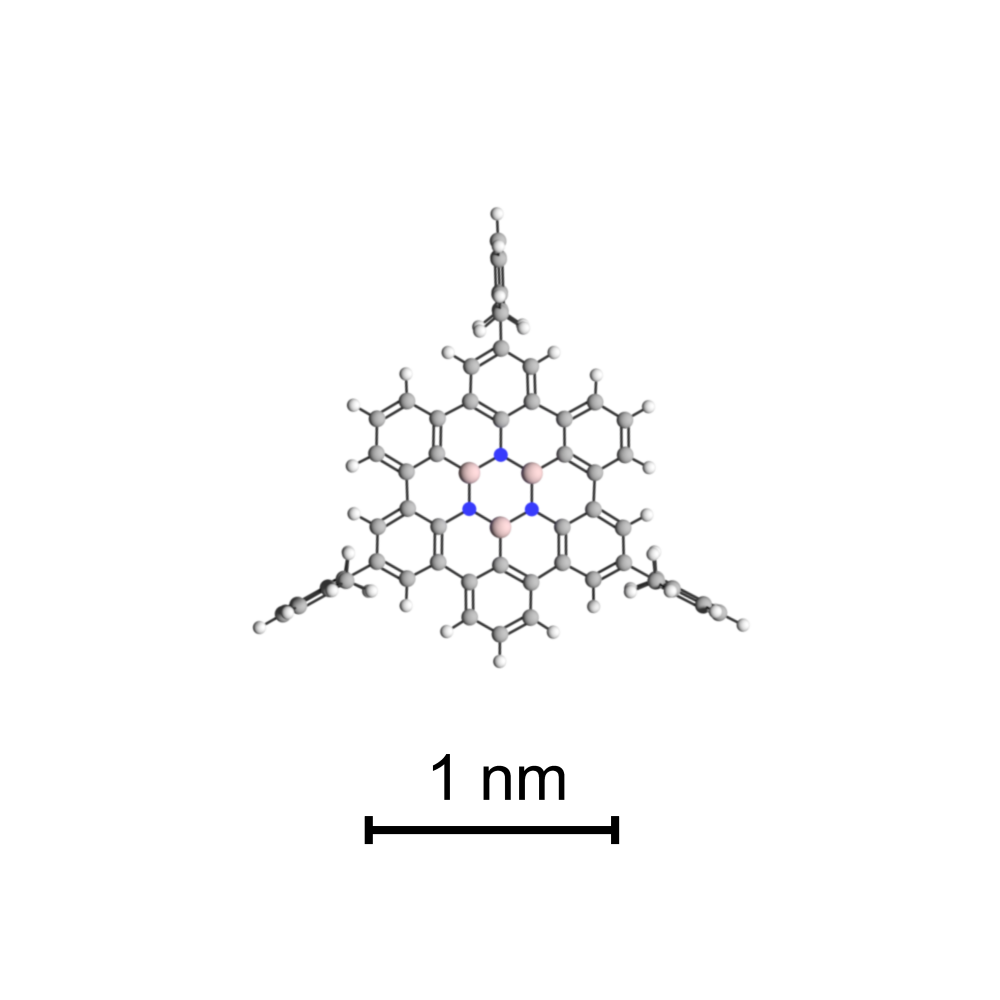
\includegraphics[width=0.45\textwidth]{./images/molecules/HBBNC-scalebar}
		\label{fig:HBBNC}
	}
	\caption{Geometric gas-phase calculated structure of \subref{fig:HBC} HBC and \subref{fig:HBBNC} HBBNC. WhileHBC is constituted solely of carbon, the central carbon ring in HBBNC is replaced with alternating boron and nitrogen atoms. Image width: \SI{4}{\nano \meter}}
	\label{fig:HBBNC+HBC}
\end{figure}

%\begin{wrapfigure}{R}{5cm}\centering
%	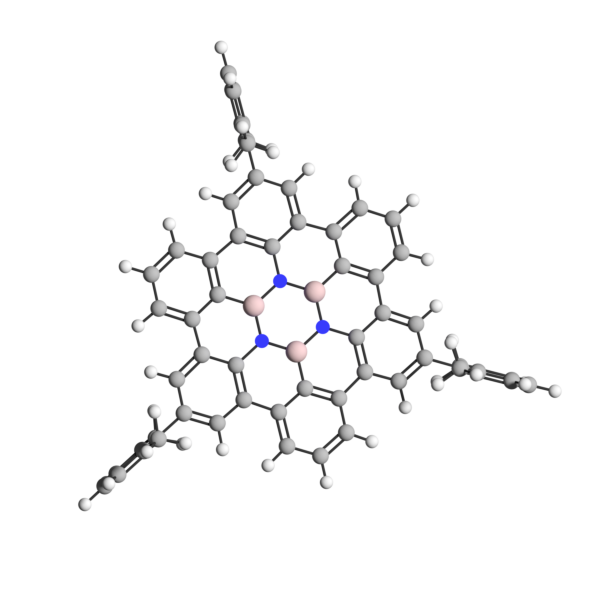
\includegraphics[angle=90,width=5cm]{./images/molecules/max-zoom/HBBNC-600}
%	\caption{HBBNC}
%	\label{fig:HBBNC-molecule}
%\end{wrapfigure}

Here we use modifications of coronene as shown in \autoref{fig:HBBNC+HBC}. For both species six benzene rings are added to extend the molecular backbone. Three 2,6-Dimethylphenyl groups were added to the molecules that now resemble a triangular footprint. While hexa‐peri‐hexabenzocoronene (HBC shown in \autoref{fig:HBC}) features a central carbon ring, it is substituted by a central borazine ring for (HBBNC shown in \autoref{fig:HBBNC}). Here the central $(BN)_3$ core is oriented to point all nitrogen atoms towards the leg functionalization.

While in 2015 \cite{Krieg_construction_2015} and 2016 \cite{Ciccullo_Quasi-Free-Standing_2016} hexy-peri-Hexabenzoborazino coronene (HBBNC) was synthesized, its bad solubility prohibited experiments. In 2017 the synthesis \cite{dosso_synthesis_2017} of a soluble, BN-doped coronene derivative by substitution of the central carbon ring was successful. 

Both species have the same number of atoms and molecular weight. The difference between both becomes apparent when calculated electronic properties are compared (in gas phase). \autoref{fig:HBC+HBBNC-electronics} contrasts the electrostatic potential (ESP) and the band gap of the two species that have been done in the group of Prof.\ Dr.\ D.\ Bonifazi. The regular covalent $sp^2$ hybridization results in an evenly distributed electron density in HBC where the central region of the molecule shows considerable negative charge as a result of the molecules central $\pi-$system. Changing the central carbon ring to a borazine ring changes the ESP. Electrons are redistributed from the central borazine ring towards the outer hexaphenylene rim. Because the bond between B and N shows an added ionic character the aromaticity is interrupted and the extended electron pi system is altered. Comparable to the difference between graphene (perfect C-C bonds, conductor) and \textit{h}-BN (ionic B-N bonds, insulator) the band gap present for HBC is \SI{0.4}{\eV} smaller than for HBBNC, changing its optoelectronic properties. By using HBBNC the HOMO-LUMO band gap could be widened and shows blue-shifted emission properties\cite{dosso_synthesis_2017} compared to its all-carbon counterpart.

\begin{figure}[]\centering
	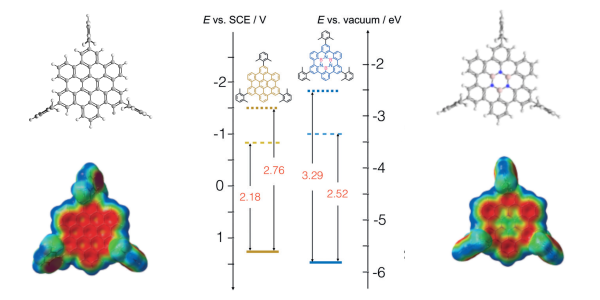
\includegraphics[width=\textwidth]{./images/dosso-combined}
	\caption{Electronic structure of HBC (left) and HBBNC (right). The even electrostatic potential (shown as colored models) for HBC is changed for HBBNC at the center where the molecule is doped with boron and nitrogen. This does deplete the electron density at the center. The electronic gap is calculated (center) and shows a smaller gap for HBC (\SI{2.18}{\eV}) compared to HBBNC (\SI{2.52}{\eV}). Adopted from \cite{dosso_synthesis_2017}}
	\label{fig:HBC+HBBNC-electronics}
\end{figure}

The present functionalization of the coronene molecule is twofold. The functionalized core of the molecule is used to create 1. an sufficiently large adsorption platform for small polar molecules (like CO) and 2. an electrostatic potential surface to trap polar species. 
%Due to the different electro negativity of the atomic species in the center adsorption of gases in the central part can be interesting effects to look out for. 
Di-Methylphenyl groups are added to lift the molecule from the substrate and guide the formation of self-assembled islands of the molecule on the surface while electronic interactions with the substrate are reduced.

Investigations with STM are performed for similar molecules on Au(111) by \cite{Krieg_construction_2015}.

\section{Results}
After RT adsorption of HBBNC on Ag(111) different assemblies are found. For low coverage the dominating pattern is a hexagon made up of six molecules in two different orientations with respect to the substrate. Although the molecule is not chiral in gas phase, adsorption on the Ag(111) surface leads to the formation an mirror image and therefore a second type of hexagon. The internal structure of these hexamers can be revealed by lateral manipulation of a hexamer with the STM tip. Three things can be concluded: 1. A hexagon is made up of six intact molecules with alternating orientations, 2. The bright features between two neighboring molecules can be attributed to rotated dimethylphenyl rings. This only occurred when two molecules are close to each other and show the right rotation, 3. Molecules not incorporated in a hexamer appear flat with no pronounced apparent height above the legs.

From the observation of smaller hexamer fragments, it seems like the growth mechanism of the hexamers is already fixed in an early state of the assembly and depends on the adsorption site of the second molecule attaching to the first. Two neighboring molecules never show the same orientation and connect to each other with parallel edges, slightly shifted.
Molecule by molecule than arranges to match the steric restrictions from the already formed hexamer. This efficient guiding mechanism leads to most molecules finish hexamer assemblies. 
Besides the dominant motif, monomers, dimers and smaller agglomerations are observed, too.

The electronic structure of single HBBNC molecules is investigated with STS after disassembly of a hexamer into its comprising single molecules. There is a pronounced electronic feature around 650 mV on the molecular center, features at \SI{1200}{\milli \volt} and \SI{1600}{\milli \volt} can be attributed to the leg and edge positions respectively. The surface state of the substrate (~ \SI{-50}{\milli \volt} next to the molecule) vanishes/shifts below the molecule. 
\begin{itemize}
	\item \textbf{\textcolor{red}{The calculated band gap of \SI{2.52}{\eV} is not observed directly because ...}}
	\item \textbf{\textcolor{red}{The fact that the band gap is not symmetric around the Fermi energy is because ...}}
	\item \textbf{\textcolor{red}{Charge transfer between molecule and substrate is possible? What would be the result? Calculate!}}
	\item \textbf{\textcolor{red}{Why/how does the surface state shift?}}
\end{itemize}

%\begin{figure}[]\centering
%	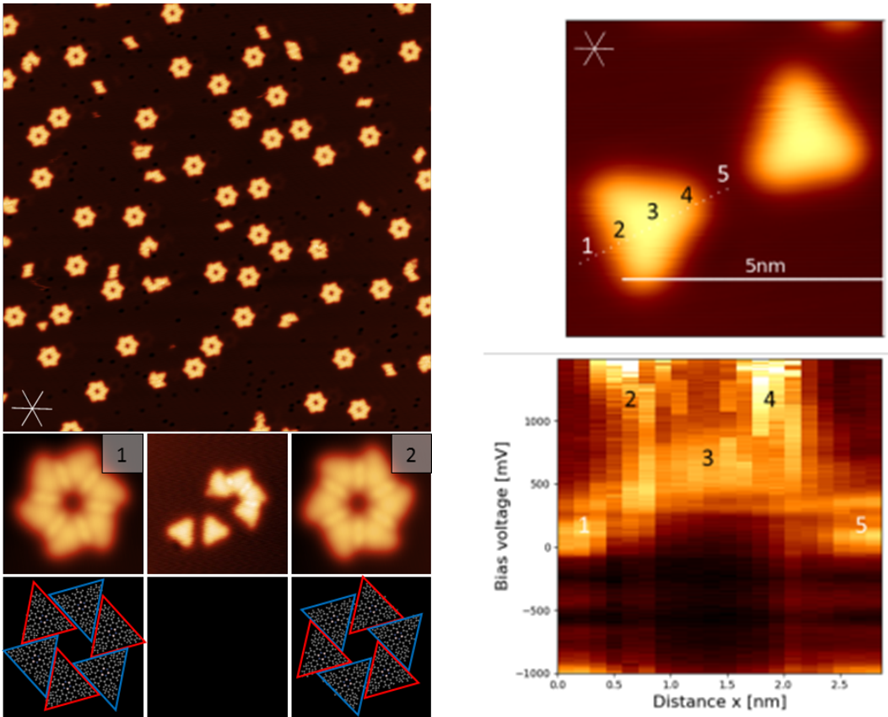
\includegraphics[width=\textwidth]{./images/test}
%	\caption{Low coverage assembly of HBBNC after RT adsorption on Ag(111). An overview image is shown on top, two hexamer orientations (1,2) are shown below. In between, lateral disassembly of e single hexamer into single molecules is shown. Last line shows molecular models for each hexamer orientation. \textcolor{red}{Imaging parameter: \SI{11.07}{\nano \meter}, \SI{1.5}{\volt}, \SI{0.1}{\nano \ampere}}. Top: STM topography: Set of spectra along the points indicated across the lower left molecule. Special points are indicated by numbers. Bottom: dI/dV spectra for each point, starting from one to five. \textcolor{red}{Renew scalebar, Imaging parameter: \SI{11.07}{\nano \meter}, \SI{1.5}{\volt}, \SI{0.1}{\nano \ampere}}.}
%	\label{fig:HBC+HBBNC-electronics}
%\end{figure}

\begin{figure}[h!]\centering
	\subfigure[Hexamer Self-Assembly after RT adsorption on Ag(111)]{
		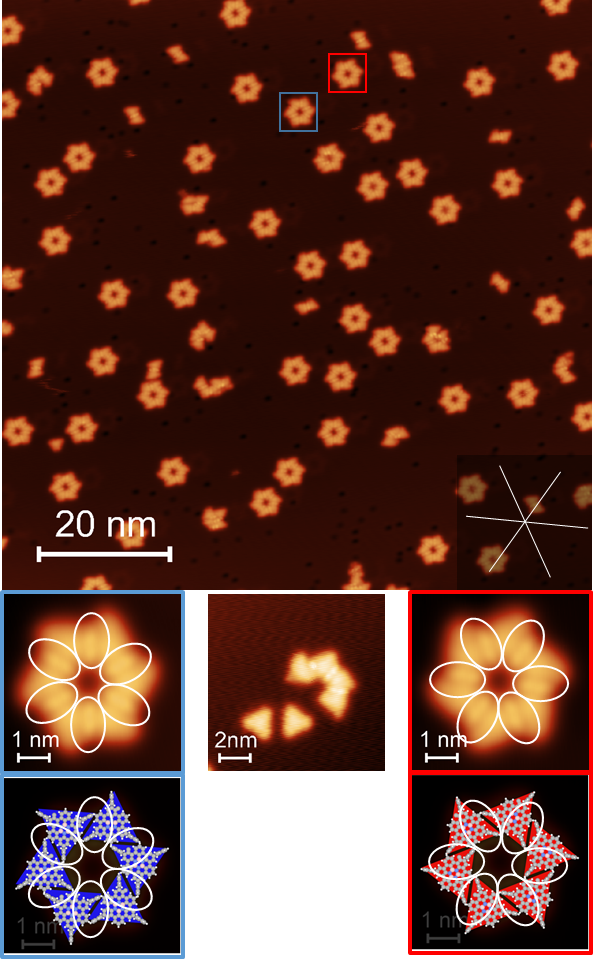
\includegraphics[height=0.7\textwidth]{./images/HBBNC-RT-assembly}
		\label{fig:HBBNC-low-coverage}
	} \quad
	\subfigure[Line spectrum for disassebled hexamer]{
		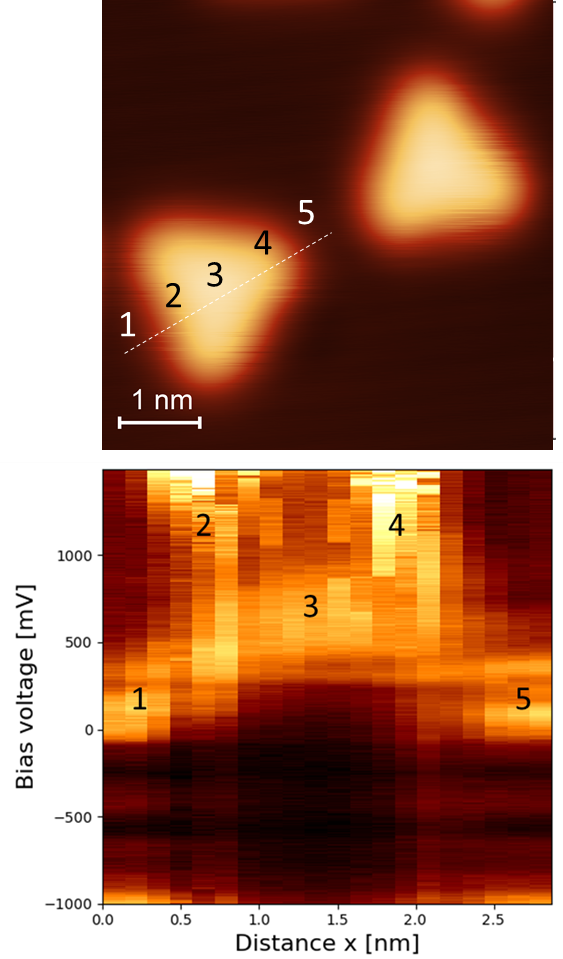
\includegraphics[height=0.7\textwidth]{./images/HBBNC-RT-spectra}
		\label{fig:HBBNC-spectra}
	}
	\caption{Low coverage RT adsorption of HBBNC on Ag(111). \subref{fig:HBBNC-low-coverage} Molecular self-assembly. An overview image is shown on top, where crystal orientation (white lines) and two hexamer orientations (red,blue) are shown. White ellipses highlight features in apparent height that do not appear for single molecules. In between, lateral disassembly of a single hexamer into single molecules is shown. Last line shows molecular models for each hexamer orientation. \subref{fig:HBBNC-spectra} STM topography (top) together with a set of spectra along the points indicated across the lower left molecule (bottom). Five points are highlighted by numbers. Bottom: dI/dV spectra for each point. Imaging parameter: \subref{fig:HBBNC-low-coverage} \SI{88.5}{\nano \meter}, \SI{750}{\milli \volt}, \SI{0.1}{\nano \ampere}, Color scale: \SIrange{0}{400}{\pico \meter}, \subref{fig:HBBNC-spectra} \SI{5.5}{\nano \meter}, \SI{750}{\milli \volt}, \SI{0.2}{\nano \ampere}, Color scale: \SIrange{0}{250}{\pico \meter}.}
	\label{fig:HBBNC-assembly-spectra}
\end{figure}

%%%%%%%%%%%%%%%%%%%%%%%%%%%%%%%%%%%%%%%
% SINGLE WRAPFIGURES 
%\begin{wrapfigure}{R}{5cm}\centering
%	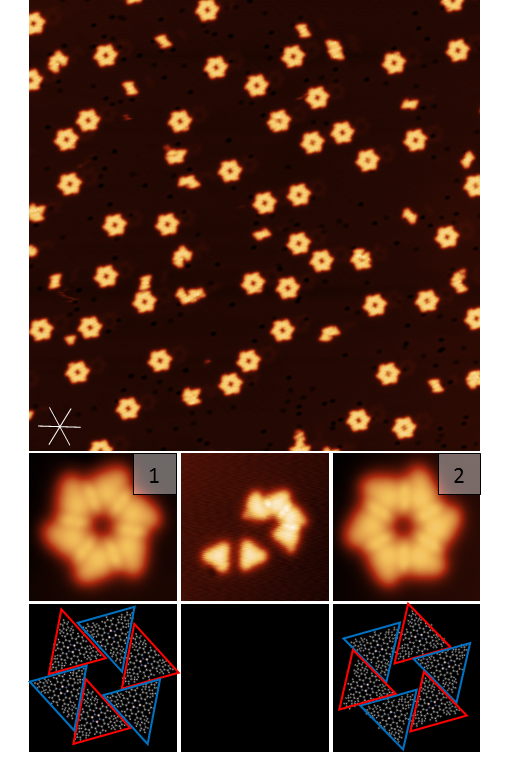
\includegraphics[width=5cm]{./images/hbbnc-ag-111-rt}
%	\caption{Low coverage assembly of HBBNC after RT adsorption on Ag(111). An overview image is shown on top, two hexamer orientations (1,2) are shown below. In between, lateral disassembly of e single hexamer into single molecules is shown. Last line shows molecular models for each hexamer orientation. \textcolor{red}{Imaging parameter: \SI{11.07}{\nano \meter}, \SI{1.5}{\volt}, \SI{0.1}{\nano \ampere}}.}
%	\label{}
%\end{wrapfigure}
%
%\begin{wrapfigure}{R}{5cm}\centering
%	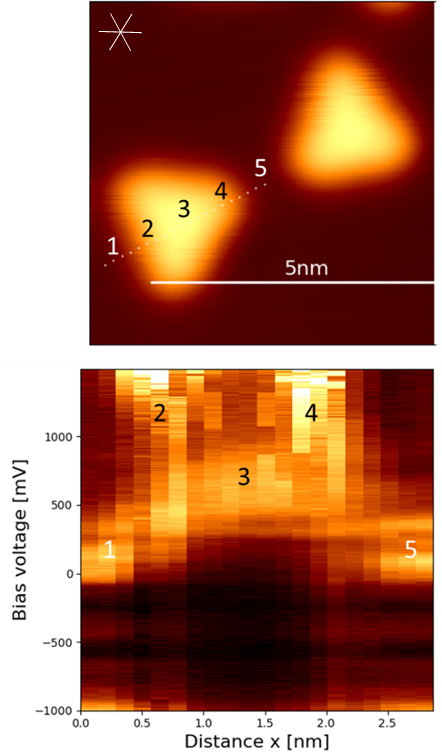
\includegraphics[width=5cm]{./images/hbbnc-ag-111-rt-linespectrum}
%	\caption{Top: STM topography: Set of spectra along the points indicated across the lower left molecule. Special points are indicated by numbers. Bottom: dI/dV spectra for each point, starting from one to five. \textcolor{red}{Renew scalebar, Imaging parameter: \SI{11.07}{\nano \meter}, \SI{1.5}{\volt}, \SI{0.1}{\nano \ampere}}.}
%	\label{}
%\end{wrapfigure}
%%%%%%%%%%%%%%%%%%%%%%%%%%%%%%%%%%%%%%%

Increasing the coverage leads to a new assembly being formed. Besides hexamers alongside their chiral counterpart form on the surface (solid and dashed blue circle), chains of dimers assemble in islands. Within these, dimer chains exist in two different orientations (solid and dashed green boxes) and are separated by single molecules (see supporting information). 
These chains are oriented along the high symmetry directions of the substrate and \SI{30}{\degree} off. Molecular orientation within the chains is slightly different than in the hexamer assemblies. Here molecules attach with a smaller lateral shift to form linear chains. 
\textbf{\textcolor{red}{Tell about binding distances and unit cell.}}
The protrusions between two neighboring molecules can be attributed to a rotation of the leg functionalization to avoid steric hindrance and to stabilize the assembly.
A second new binding motif is observed (white square).  It is made up of four molecules, whose close proximity in the center form a pattern reminiscent of a clover-leaf. It can be seen that (in contrast to hexamers) molecules can attach to the rims and evolve into more extended structures.

\begin{figure}[] \centering
	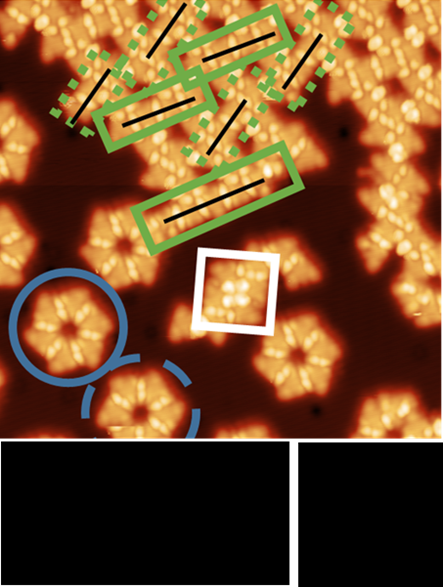
\includegraphics[width=0.7\textwidth]{./images/hbbnc-ag-111-rt-med-coverage}
	\caption{Medium coverage adsorption of HBBNC at RT on Ag(111). While the chiral assemblies are still pressent (blue circles), additional binding motifs like chains (green boxes) and squares (white box) occur. \textcolor{red}{Scalebar, Imaging parameter: \SI{11.07}{\nano \meter}, \SI{1.5}{\volt}, \SI{0.1}{\nano \ampere}}.}
	\label{}
\end{figure}

Further increasing the coverage results in dense regions being formed. The dominating pattern is the clover-leaf rarely observed in the medium coverage phase. It is present here in two different orientations (white and blue box) and distributed such that neighboring squares do not show the same orientation. Two squares with the same orientation (white/blue) are separated by lines made up of four bright spots aligned parallel to the square edge. Squares with different rotations do not show these connections between them, but a single protrusion with larger apparent height.
Binding motif, binding distances.

\begin{figure}[] \centering
	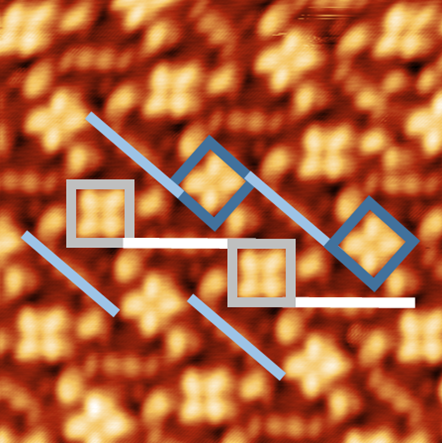
\includegraphics[width=0.7\textwidth]{./images/hbbnc-ag-111-rt-high-coverage}
	\caption{High coverage adsorption of HBBNC at RT on Ag(111). Two different orientations of a repeating binding motif is emphasized by STM topography images and marked with two color sets (blue/grey). \textcolor{red}{Scalebar, Imaging parameter: \SI{11.07}{\nano \meter}, \SI{1.5}{\volt}, \SI{0.1}{\nano \ampere}}.}
	\label{}
\end{figure}

A sample prepared at RT has been annealed to \SI{350}{\celsius} and \SI{420}{\celsius}.

After the sample is annealed to \SI{350}{\celsius} only monomers and few random agglomerates are imaged on the surface. Although the molecules undergo the same temperature range where hexamers are formed (from RT to \SI{5}{\kelvin}) no regular assembly is imaged. Because the assembly is guided by the presence of the dimethylphenyl group a closer look to the molecular conformation is taken. Three different types can be distinguished. 1: Flat molecules, 2: Molecules with a single protrusion close to the leg position, 3: Molecules with a leg missing.

The unstable imaging conditions above some of the molecules legs indicate their flexibility while the others seem to be rigidly connected to the molecular backbone and therefor imaged stable. The vanishing hexagon binding motif - observed for the un-annealed sample - underpins the importance for the molecules leg to adopt the assembly. This flexibility of all legs is not present any more after annealing to \SI{350}{\celsius} and hexamer formation is suppressed. Molecular orientation?
Increasing the annealing temperature to \SI{420}{\celsius} results in a percolated network where monomers present at \SI{350}{\celsius} coalesce and connect via their legs. Lateral manipulation attempts have been done, showing a stiff connection between neighboring molecules. Opposing to the previous preparations, the assembly could not be divided into single monomers. This rigid connection indicates a covalent coupling of the molecules. 
Molecular orientation?

\begin{figure}[] \centering
	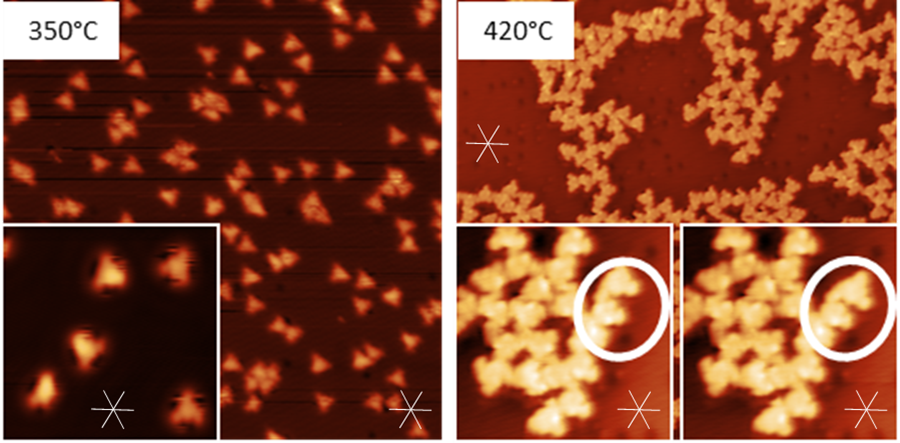
\includegraphics[width=0.7\textwidth]{./images/hbbnc-ag-111-annealed}
	\caption{Annealing steps of HBBNC on Ag(111) after RT adsorption. Left: After annealing to \SI{350}{\celsius} and cooling down to LT-STM temperatures no hexamers are visible. A variety of molecular orientations and different conformations are present (inset). Right: Annealing the same sample to \SI{420}{\celsius} leads to an unregular network where molecules are connected via their legs and not separable by lateral manipulation. \textcolor{red}{Scalebar, Imaging parameter: \SI{11.07}{\nano \meter}, \SI{1.5}{\volt}, \SI{0.1}{\nano \ampere}}.}
	\label{}
\end{figure}

Since the formation of a new bond is expected to change the core levels of participating elements (Carbon, C\textit{1s}), XPS measurements are done and presented in the following.

Preparations have been done to further investigate the connection between molecules annealed to \SI{420}{\celsius}. Sub-ML as well as multilayer preparations have been annealed to \SI{420}{\celsius} to quantify the change in binding energy. After RT deposition of a sub-ML HBBNC on Ag(111) a single C\textit{1s} peak is observed that grows with increasing coverage but maintains its position.
Is there no shift after adsorption of a multilayer?
After annealing a multilayer preparation the C 1s position shifts to lower binding energies by (~\SI{1}{\eV}), a behavior typical for cyclodehydrogenation and ring closure reactions of e.g. porphyrins \textcolor{red}{(\textbf{citation})}. \textcolor{red}{(\textbf{What are other mechanisms for a shift towards lower binding energies => screening should change in monolayer/multilayer regimes?}} The area below the peak drops to a sub-ML coverage, a clear indication for desorption of the second and third layer. A covalently coupled layer would not desorp, so coupling in the lowest layer takes place after multilayer desorption.
It can be concluded that annealing HBBNC on a Ag(111) surface leads to the formation of a covalent network stabilized via covalent bonds formed across the legs.

\begin{figure}[] \centering
	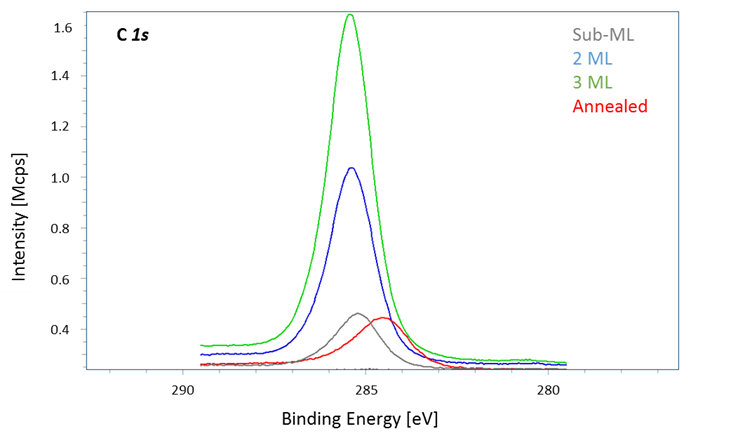
\includegraphics[width=0.7\textwidth]{./images/hbbnc-xps1}
	\caption{XPS C\textit{1s} spectra of HBBNC adsorbed on Ag(111) for increasing coverages. Annealing to \SI{420}{\celsius} leads to a decrease in signal and shift to lower binding energies.}
	\label{}
\end{figure}

To further check the conformational changes in the molecule after annealing, AFM measurements are done. nc-AFM has the big advantage over STM that it is less sensible to electronic changes in the molecule – more closely resembling the true geometric shape.

Nc-AFM measurements are a complementary method to investigate the molecules before and after annealing to \SI{420}{\celsius}. 

\textbf{Before annealing} the adsorption geometry of monomers is investigated. By scanning the same molecule in different heights, elevated parts of the molecule can be easily distinguished by their larger interaction force with the tip (the involved larger frequency shift is shown as protrusion in nc-AFM images). In contrast to STM measurement where no obvious change in apparent height was observed at RT between legs, AFM measurements show that the dimethylphenyl legs of a monomer do not lie flat on the surface but have an elevated and lower lying part. While the initial orientation on the surface is likely determined at adsorption, the legs are able to rotate under the influence of the AFM tip (see SI).

\textbf{After annealing} \textcolor{red}{IS that a bond? What does the contrast mean? CITE; CITE, CITE}
The triangular molecules that appeared flat in STM (after annealing to \SI{420}{\celsius}) reveal their interesting geometric properties when investigated by means of nc-AFM. It is observed that many of the molecules appear to have their dimethylphenyl groups aligned planar to the surface. A behavior expected for a ring closure reaction between the hexabenzol groups and dimethylphenyl legs. EXAMPLES for AFM showing that in other systems. In the present case, almost all molecules showed some defined contrast in the connection region. DISCUSS distances, directions and excess of carbon rings.
When the legs rotate parallel to the surface, the molecular backbone comes closer to the metal => charge transfer/screening and such things!!

\begin{figure}[] \centering
	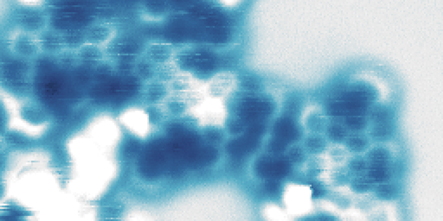
\includegraphics[width=0.7\textwidth]{./images/hbbnc-annealed-afm}
	\caption{AFM image displaying the Laplace filtered frequency shift channel. While rings constituting the molecule are visible, features in between rigid molecular connection are visible. \textcolor{red}{Scalebar, Imaging parameter: \SI{11.07}{\nano \meter}, \SI{1.5}{\volt}, \SI{0.1}{\nano \ampere}}.}
	\label{}
\end{figure}

To have the molecule adsorbed more even on the surface, another substrate is chosen. Silver is known to have a larger impact on adsorption geometries than Au(111) has (bowl shape of PAH on Ag(111) \textcolor{red}{=> CITE!}).

In contrast to adsorption on Ag(111) where almost all molecules are incorporated into hexamers, molecules separate into monomers on Au(111). Molecules follow the herringbone reconstruction visible as bright stripes in the STM image. 
(These divide the surface into regions of fcc and hcp reconstruction.
Which one is broad, which one is small)
Molecules show two different appearances. While some appear to adsorb flat in STM, others already show a protrusion above one of their legs. This protrusion is not caused by parts of the herringbone reconstruction, two molecules on very similar adsorption sites within the reconstruction show different appearances.
\textcolor{red}{\textbf{What are conformational changes here?}}

\begin{figure}[] \centering
	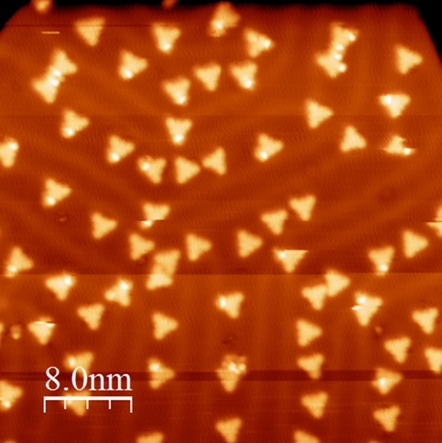
\includegraphics[width=0.5\textwidth]{./images/hbbnc-au-111-rt}
	\caption{STM topography image of HBBNC on Au(111)/Mica. \textcolor{red}{\textbf{Stripes}} of the herringbone reconstruction divide the surface into regions of fcc and hcp stacking order. Only monomers form after adsorption at RT. \textcolor{red}{Scalebar, Imaging parameter: \SI{11.07}{\nano \meter}, \SI{1.5}{\volt}, \SI{0.1}{\nano \ampere}}.}
	\label{}
\end{figure}

\section{Summary \& Discussion}
It is reported that for HBC, no stable second layer of molecules can be found for a strong electron donor like HBC \cite{de_feyter_two-dimensional_2003}.

\section{Conclusion}